% \documentclass[table]{beamer}
\documentclass[table,handout]{beamer}
\setbeameroption{show notes}
% \setbeameroption{hide notes}
% \setbeameroption{show only notes}
\usepackage{varwidth}

\newif\ifhide
\newif\ifpost
\newif\ifhideclicker

% \hidetrue
% \hideclickertrue
% \posttrue

\newcommand{\whiteout}[1]{\textcolor{white}{#1}}
% \newcommand{\whiteoutbox}[1]{\fcolorbox{white}{white}{\parbox{\dimexpr \linewidth-2\fboxsep-2\fboxrule}{\whiteout{#1}}}}
% \newcommand{\notebox}[1]{\fcolorbox{blue}{white}{\parbox{\dimexpr \linewidth-2\fboxsep-2\fboxrule}{#1}}}
\newcommand{\whiteoutbox}[1]{\fcolorbox{white}{white}{\parbox{\linewidth}{\whiteout{#1}}}}
\newcommand{\notebox}[1]{\fcolorbox{blue}{white}{\parbox{\linewidth}{#1}}}
\newcommand{\blankbox}[1]{\phantom{\varwidth{\linewidth}\whiteoutbox{#1}\endvarwidth}}
\newcommand{\blank}[1]{\phantom{\varwidth{\linewidth}#1\endvarwidth}}

\ifhide%
    \newcommand{\hmask}[1]{\blank{#1}}%
\else%
    \newcommand{\hmask}[1]{#1}%
\fi

\ifhide%
    \newcommand{\wout}[1]{\whiteout{#1}}%
\else%
    \newcommand{\wout}[1]{#1}%
\fi

\ifhide%
    \newcommand{\hignore}[1]{}%
\else%
    \newcommand{\hignore}[1]{#1}%
\fi

\ifpost%
    \newcommand{\nopost}[1]{}%
\else%
    \newcommand{\nopost}[1]{#1}%
\fi

\ifhideclicker%
    \newcommand{\clickerslide}[1]{\stepcounter{clickerQuestionCounter}%
        \begin{frame}[t]
            \textcolor{blue}{Q \arabic{clickerQuestionCounter}:}
        \end{frame}}
\else%
    \newcommand{\clickerslide}[1]{#1}%
\fi

\ifhide%
    \newcommand{\hidebox}[1]{\blank{#1}}%
\else%
    \newcommand{\hidebox}[1]{\notebox{#1}}%
\fi

\ifhide%
    \newcommand{\wbox}[1]{\whiteoutbox{#1}}%
\else%
    \newcommand{\wbox}[1]{\notebox{#1}}%
\fi

\ifhide%
    \newcommand{\nbox}[1]{\blankbox{#1}}%
\else%
    \newcommand{\nbox}[1]{\notebox{#1}}%
\fi

\ifhideclicker%
    \newcommand{\clickeranswer}[1]{#1}%
\else%
    \ifhide%
        \newcommand{\clickeranswer}[1]{#1}%
    \else%
        \newcommand{\clickeranswer}[1]{\textbf{\textcolor{blue}{#1}}}%
    \fi
\fi

\usepackage{beamerthemesplit}
% \usetheme{boxes}
\usetheme{Malmoe}
\usecolortheme{seahorse}
% \usecolortheme{seagull}
\usepackage{ifthen}
\usepackage{xspace}
\usepackage{multirow}
\usepackage{multicol}
\usepackage{booktabs}
\usepackage{xcolor}
\usepackage{wasysym}
\usepackage{comment}
\usepackage{hyperref}
\hypersetup{pdfborder={0 0 0}, colorlinks=true, urlcolor=blue, linkcolor=blue, citecolor=blue}
\usepackage{changepage}
\usepackage[compatibility=false]{caption}
\captionsetup[figure]{font=scriptsize, labelformat=empty, textformat=simple, justification=centering, skip=2pt}
\usepackage{tikz}
\usetikzlibrary{trees,calc,backgrounds}

\usepackage[bibstyle=joaks-slides,maxcitenames=3,mincitenames=1,backend=biber]{biblatex}

\newrobustcmd*{\shortfullcite}{\AtNextCite{\renewbibmacro{title}{}\renewbibmacro{in:}{}\renewbibmacro{number}{}}\fullcite}

\newrobustcmd*{\footlessfullcite}{\AtNextCite{\renewbibmacro{title}{}\renewbibmacro{in:}{}}\footfullcite}

% Make all footnotes smaller
% \renewcommand{\footnotesize}{\scriptsize}

\definecolor{myGray}{gray}{0.9}
\colorlet{rowred}{red!30!white}

\setbeamertemplate{blocks}[rounded][shadow=true]

\setbeamercolor{defaultcolor}{bg=structure!30!normal text.bg,fg=black}
\setbeamercolor{block body}{bg=structure!30!normal text.bg,fg=black}
\setbeamercolor{block title}{bg=structure!50!normal text.bg,fg=black}

\newenvironment<>{varblock}[2][\textwidth]{%
  \setlength{\textwidth}{#1}
  \begin{actionenv}#3%
    \def\insertblocktitle{#2}%
    \par%
    \usebeamertemplate{block begin}}
  {\par%
    \usebeamertemplate{block end}%
  \end{actionenv}}

\newenvironment{displaybox}[1][\textwidth]
{
    \centerline\bgroup\hfill
    \begin{beamerboxesrounded}[lower=defaultcolor,shadow=true,width=#1]{}
}
{
    \end{beamerboxesrounded}\hfill\egroup
}

\newenvironment{onlinebox}[1][4cm]
{
    \newbox\mybox
    \newdimen\myboxht
    \setbox\mybox\hbox\bgroup%
        \begin{beamerboxesrounded}[lower=defaultcolor,shadow=true,width=#1]{}
    \centering
}
{
    \end{beamerboxesrounded}\egroup
    \myboxht\ht\mybox
    \raisebox{-0.25\myboxht}{\usebox\mybox}\hspace{2pt}
}

\newenvironment{mydescription}{
    \begin{description}
        \setlength{\leftskip}{-1.5cm}}
    {\end{description}}

\newenvironment{myitemize}{
    \begin{itemize}
        \setlength{\leftskip}{-.3cm}}
    {\end{itemize}}

% footnote without a marker
\newcommand\barefootnote[1]{%
  \begingroup
  \renewcommand\thefootnote{}\footnote{#1}%
  \addtocounter{footnote}{-1}%
  \endgroup
}

% define formatting for footer
\newcommand{\myfootline}{%
    {\it
    \insertshorttitle
    \hspace*{\fill} 
    \insertshortauthor, \insertshortinstitute
    % \ifx\insertsubtitle\@empty\else, \insertshortsubtitle\fi
    \hspace*{\fill}
    \insertframenumber/\inserttotalframenumber}}

% set up footer
\setbeamertemplate{footline}{%
    \usebeamerfont{structure}
    \begin{beamercolorbox}[wd=\paperwidth,ht=2.25ex,dp=1ex]{frametitle}%
        % \Tiny\hspace*{4mm}\myfootline\hspace{4mm}
        \tiny\hspace*{4mm}\myfootline\hspace{4mm}
    \end{beamercolorbox}}

% remove navigation bar
\beamertemplatenavigationsymbolsempty

\makeatletter
    \newenvironment{noheadline}{
        \setbeamertemplate{headline}[default]
        \def\beamer@entrycode{\vspace*{-\headheight}}
    }{}
\makeatother

\newcounter{clickerQuestionCounter}
\ifhideclicker%
\newenvironment{clickerquestion}
{ \stepcounter{clickerQuestionCounter}
  \begin{enumerate}[Q \arabic{clickerQuestionCounter}:]\color{white} }
{ \end{enumerate} }
\else%
\newenvironment{clickerquestion}
{ \stepcounter{clickerQuestionCounter}
  \begin{enumerate}[Q \arabic{clickerQuestionCounter}:] }
{ \end{enumerate} }
\fi

\ifhideclicker%
\newenvironment{clickeroptions}
{ \begin{enumerate}[\begingroup\color{white} 1)\endgroup]\color{white} }
{ \end{enumerate} }
\else%
\newenvironment{clickeroptions}
{ \begin{enumerate}[\begingroup\color{red} 1)\endgroup] }
{ \end{enumerate} }
\fi


\tikzstyle{centered} = [align=center, text centered, font=\sffamily\bfseries]
\tikzstyle{skip} = [centered, inner sep=0pt, fill]
\tikzstyle{empty} = [centered, inner sep=0pt]
\tikzstyle{inode} = [centered, circle, minimum width=4pt, fill=black, inner sep=0pt]
\tikzstyle{tnode} = [centered, circle, inner sep=1pt]
\tikzset{
  % edge styles
  level distance=10mm,
  mate/.style={edge from parent/.style={draw,distance=3pt}},
  mleft/.style={grow=left, level distance=10mm, edge from parent path={(\tikzparentnode.west)--(\tikzchildnode.east)}},
  mright/.style={grow=right, level distance=10mm, edge from parent path={(\tikzparentnode.east)--(\tikzchildnode.west)}},
  % node styles
  male/.style={rectangle,minimum size=4mm,fill=gray!80},
  female/.style={circle,minimum size=4mm,fill=gray!80},
  amale/.style={male,fill=red},
  afemale/.style={female,fill=red},
}

\newcommand{\highlight}[1]{\textcolor{violet}{\textit{\textbf{#1}}}}
\newcommand{\super}[1]{\ensuremath{^{\textrm{\sffamily #1}}}}
\newcommand{\sub}[1]{\ensuremath{_{\textrm{\sffamily #1}}}}
\newcommand{\dC}{\ensuremath{^\circ{\textrm{C}}}}
\newcommand{\tb}{\hspace{2em}}
\providecommand{\e}[1]{\ensuremath{\times 10^{#1}}}
\newcommand{\myHangIndent}{\hangindent=5mm}

\newcommand{\spp}[1]{\textit{#1}}

\newcommand\mybullet{\leavevmode%
\usebeamertemplate{itemize item}\hspace{.5em}}

\makeatletter
\newcommand*{\rom}[1]{\expandafter\@slowromancap\romannumeral #1@}
\makeatother

\newcommand{\blankslide}{{\setbeamercolor{background canvas}{bg=black}
\setbeamercolor{whitetext}{fg=white}
\begin{frame}<handout:0>[plain]
\end{frame}}}

\newcommand{\whiteslide}{
\begin{frame}<handout:0>[plain]
\end{frame}}

\newcommand{\f}[1]{\ensuremath{F_{#1}}}
\newcommand{\x}[1]{X\ensuremath{^{#1}}}
\newcommand{\y}[1]{Y\ensuremath{^{#1}}}

% Population growth macros
\newcommand{\popsize}[1]{\ensuremath{N_{#1}}}
\newcommand{\popgrowthratediscrete}[1]{\ensuremath{\lambda_{#1}}}
\newcommand{\popgrowthrate}[1]{\ensuremath{r_{#1}}}
\newcommand{\ptime}{\ensuremath{t}\xspace}

\tikzset{hide on/.code={\only<#1>{\color{white}}}}
\tikzset{
    invisible/.style={opacity=0},
    visible on/.style={alt={#1{}{invisible}}},
    alt/.code args={<#1>#2#3}{%
        \alt<#1>{\pgfkeysalso{#2}}{\pgfkeysalso{#3}}
        % \pgfkeysalso doesn't change the path
    },
}

\bibliography{../bib/references}
\author[J.\ Oaks]{
    %Jamie R.\ Oaks\inst{1}
    Jamie R.\ Oaks
}
\institute[BIOL 180]{
    \inst{}%
        BIOL 180: Introductory Biology
}



\title[Gene flow \& inbreeding]{Gene Flow \& Inbreeding}
% \date{\today}
\date{April 28, 2015}

\begin{document}

\begin{noheadline}
\maketitle
\end{noheadline}

\nopost{
\begin{noheadline}
\begin{frame}[c]
    \vspace{-6mm}
    \begin{center} 
        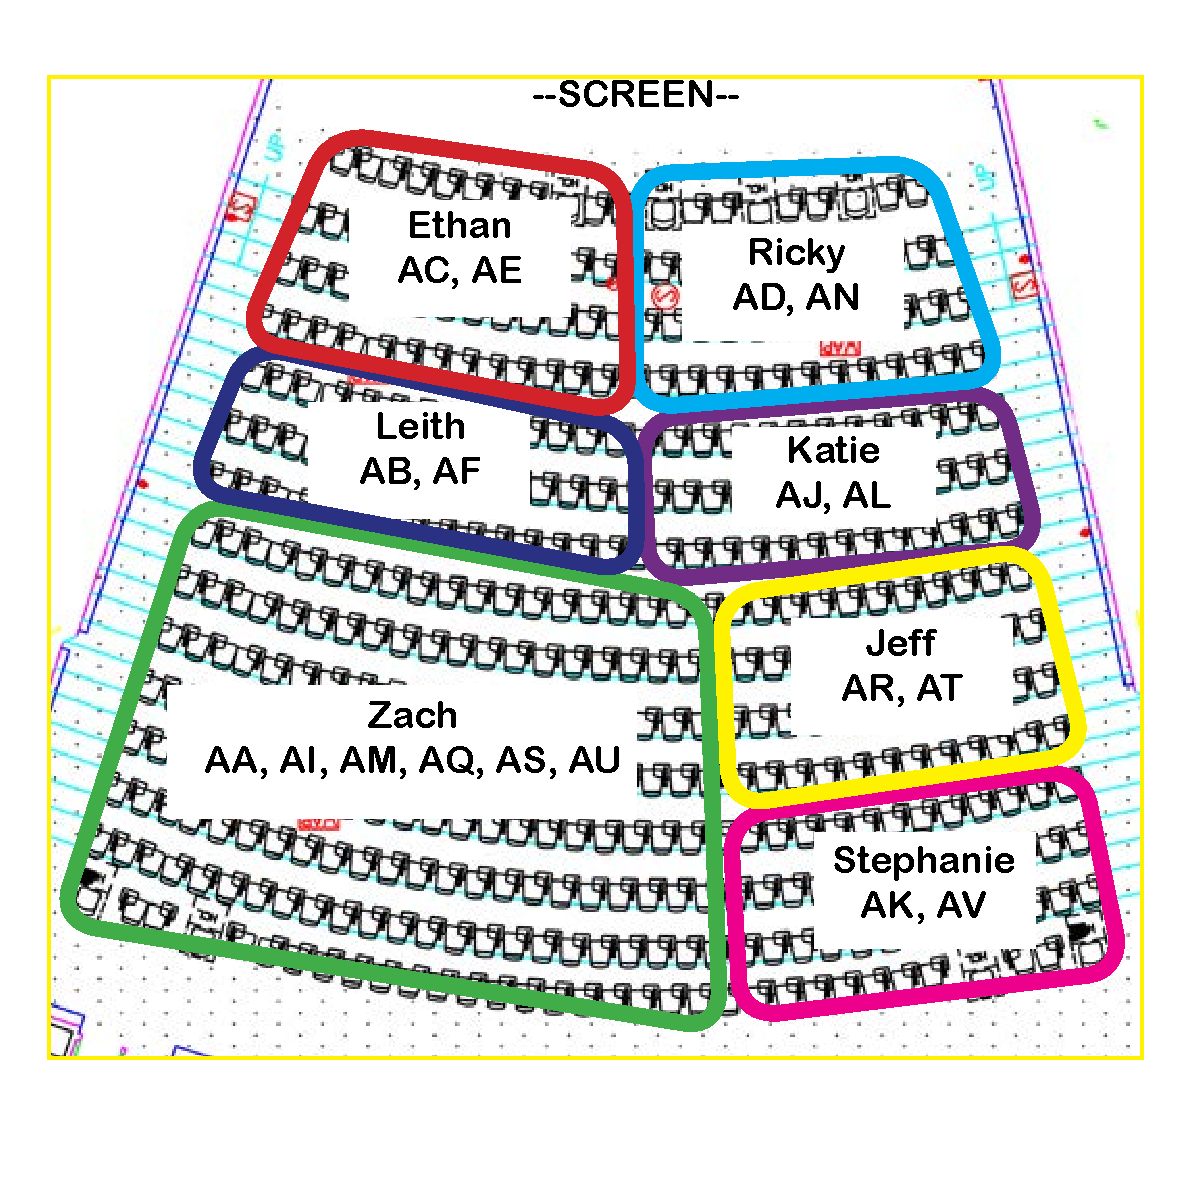
\includegraphics[height=1.2\textheight]{../images/seating-chart.pdf}
    \end{center}
\end{frame}
\end{noheadline}
}

\clickerslide{
\begin{noheadline}
\begin{frame}
    \begin{adjustwidth}{-1.5em}{-1.5em}
    \begin{clickerquestion}
        \item Assume that mutations occur at a rate of 0.0001 per gene per
            generation. On average, how long would it take mutation alone to
            create a 1\% change in allele frequencies at a gene in \textit{C.\
                elegans}, with a generation time of 4 days, and \textit{E.\
                coli}, with a generation time of 20 minutes? 
    \end{clickerquestion}
    \begin{table}%[htbp]
        % \addtolength{\tabcolsep}{-0.09cm}
        \centering
        \begin{tabular}{ l c c }
             & \textit{C.\ elegans} & \textit{E.\ coli} \\
            \hline
            \textcolor{red}{1)} & 4 days & 20 minutes \\ 
            \textcolor{red}{2)} & 40 days & 200 minutes \\ 
            \textcolor{red}{3)} & \clickeranswer{$\approx$1.1 years} &
            \clickeranswer{$\approx$33 hours} \\ 
            \textcolor{red}{4)} & $\approx$11 years & $\approx$14 days \\ 
            \textcolor{red}{5)} & \multicolumn{2}{l}{It depends on the number of genes in the genome} \\ 
        \end{tabular}
    \end{table}

    \nbox{$\frac{0.01 \,\textrm{mutations/gene}}{0.0001
            \,\textrm{mutations/gene/generation}} = 100 \,\textrm{generations}$
        \\
        \textit{C.\ elegans}: $100 \,\textrm{generations} \times 4
        \,\textrm{days/generation} = 400 \,\textrm{days} \approx 1.1
        \,\textrm{years}$ \\
        \textit{E.\ coli}: $100 \,\textrm{generations} \times 20
        \,\textrm{hours/generation} = 2000 \,\textrm{minutes} \approx 33
        \,\textrm{hours}$}
    \end{adjustwidth}
\end{frame}
\end{noheadline}
}

\begin{noheadline}
\begin{frame}
\frametitle{Today's issues:}
\vspace{5mm}
\tableofcontents[subsectionstyle=hide]
\end{frame}
\end{noheadline}

\section[How gene flow changes allele frequencies]{How does gene flow cause
    changes in allele frequencies?}

\begin{frame}[t]
    \frametitle{Gene flow: The one-island model}
    \begin{adjustwidth}{-1.5em}{-1.5em}
        \vspace{-4mm}
        Model: One-way movement of individuals (and their alleles) from a large
        population on a continent to a small population on an island.

        \begin{itemize}
            \item<2-> Suppose that allele $A_1$ is at frequency 1.0 on an
                island with 400 individuals.

            % \vspace{1mm}
            \item<3-> Suppose that allele $A_2$ is at frequency 1.0 on the
                continent.

            % \vspace{1mm}
            \item<4-> If 100 individuals from the continent migrate to the
                island, the frequencies of alleles in the island populations
                are now (the species is diploid):
        \end{itemize}

        \nbox{$fr(A_2) = \frac{100 \times 2}{1000} = 0.2$ \\
              $fr(A_1) = \frac{400 \times 2}{1000} = 0.8$} 

    
        \uncover<5->{
        \vspace{1.7cm}
        \textbf{Punchline:} Evolution has occurred because of gene flow!
        }

    \end{adjustwidth}
\end{frame}

\begin{frame}[t]
    \frametitle{What are the evolutionary consequences of gene flow?}
    \begin{adjustwidth}{-1.5em}{-1.5em}
        \begin{itemize}
        \vspace{-4mm}
            \item Genetically, does it make populations more alike, more
                dissimilar, or no impact?

                \nbox{More alike. For example, on the last slide, the island
                    population is more similar to the continent population
                    after migration occurred.}

                \vspace{1cm}
            \item In the recipient population, does it increase fitness,
                decrease fitness, or no impact?

                \nbox{You can't tell---it depends on the alleles that
                    arrive and the environment}

                \vspace{1cm}
            \item How is gene flow affecting human populations?

                \nbox{It is homogenizing populations}

        \end{itemize}
    \end{adjustwidth}
\end{frame}

\clickerslide{
\begin{frame}
    \begin{clickerquestion}
        \item How do founder effects and gene flow differ?
        \begin{clickeroptions}
            \item Compared to a founder effect, less genetic drift occurs
                during gene flow.
            \item Gene flow is much more common; founder effects usually only
                occur on islands. 
            \item \clickeranswer{Founder effects don't add alleles to an
                    existing population.}
            \item They are two sides to the same coin (have similar or
                identical effects). 
        \end{clickeroptions}
    \end{clickerquestion}
\end{frame}
}

\clickerslide{
\begin{frame}
    \begin{clickerquestion}
        \item Deforestation and suburbanization are forcing wild populations
            into isolated fragments of habitat. How will these isolated
            populations change over time relative to each other, due to REDUCED
            gene flow? 

        \begin{clickeroptions}
            \item Less distinct: mutation, selection, and drift would make
                allele frequencies converge (become more similar). 
            \item No (or little) change: mutation, selection, and drift in the
                various populations would balance out. 
            \item The result is not predictable---it depends on the
                environment. 
            \item \clickeranswer{More distinct: mutation, selection, and drift
                    would act independently in each.}
        \end{clickeroptions}
    \end{clickerquestion}
\end{frame}
}

\section[How non-random mating changes genotype frequencies]{How do inbreeding
    and other forms of non-random mating cause changes in genotype
    frequencies?}

\begin{frame}[t]
    \begin{adjustwidth}{-1.5em}{-1.5em}
        \textcolor{blue}{\bf How do inbreeding and other forms of non-random
            mating cause changes in genotype frequencies?}

        \vspace{2mm}
        Consider selfing---an extreme form of inbreeding

        \begin{table}
            \centering
            \begin{tabular}{l l c r }
                Generation & & & \\
                0 & $A_1A_1$ & $A_1A_2$ & $A_2A_2$ \\[1ex]
                1 & & \wout{$\;\;\;\; \leftarrow \frac{1}{4}A_1A_1; \frac{1}{2}A_1A_2;
                 \frac{1}{4}A_2A_2 \rightarrow \;\;\;\;$} & \\[1ex]
                2 & & \wout{$\;\;\;\; \leftarrow \frac{1}{4}A_1A_1; \frac{1}{2}A_1A_2;
                 \frac{1}{4}A_2A_2 \rightarrow \;\;\;\;$} & \\[1ex]
                3 & & \wout{$\;\;\;\; \leftarrow \frac{1}{4}A_1A_1; \frac{1}{2}A_1A_2;
                 \frac{1}{4}A_2A_2 \rightarrow \;\;\;\;$} & \\
                 & & & \\
            \end{tabular}
        \end{table}

        \begin{enumerate}
            \item How does inbreeding affect allele frequencies?

                \nbox{Inbreeding alone does NOT affect allele frequencies}

            \item How does inbreeding affect genotype frequencies?

                \nbox{Inbreeding increases the frequency of homozygotes and
                    decreases the frequency of heterozygotes}
        \end{enumerate}
    \end{adjustwidth}
\end{frame}

\begin{frame}[t]
    \begin{adjustwidth}{-1.5em}{-1.5em}
        Why does inbreeding depression occur?

        \begin{itemize}
            \item Deleterious recessive alleles are usually at low frequency, so most
                are found in \ldots

                \nbox{If an allele is rare, it is unlikely for an individual to
                    inherit two copies by chance alone, and so it will most
                    likely be found in heterozygotes. Also, given the allele is
                    deleterious and recessive, it is even less likely to find
                    an individuals with two copies, due to selection; the
                    allele will tend to ``hide out'' from selection in
                    heterozygotes}  

            \item BUT, inbreeding increases the proportion of homozygous
                recessive individuals, so \ldots

                \nbox{When there is inbreeding, more individuals will have two
                    copies of the deleterious recessive. Thus, more individuals
                    will exhibit low-fitness phenotypes when there is
                    inbreeding. I.e., inbreeding can decrease average fitness.}
        \end{itemize}
    \end{adjustwidth}
\end{frame}

\clickerslide{
\begin{frame}
    \begin{clickerquestion}
        \item Why do small populations become inbred?

        \begin{clickeroptions}
            \item They are usually stable or declining in size. 
            \item \clickeranswer{Eventually, all individuals in small
                    populations are closely related.}
            \item Founder events establish populations in new, previously
                unoccupied habitats.
            \item Population bottlenecks cause large changes in allele
                frequencies.
        \end{clickeroptions}
    \end{clickerquestion}
\end{frame}
}

\clickerslide{
\begin{frame}
    \begin{clickerquestion}
        \item In some species, inbreeding via self-fertilization occurs
            routinely, but no inbreeding depression is observed. How is this
            possible? 

        \begin{clickeroptions}
            \item \clickeranswer{Deleterious recessives have been eliminated
                    via intense selection in the past.}
            \item The observed phenotypic variation is due to gene $\times$
                environment interactions.
            \item The traits involved are polygenic.
            \item Most individuals in the population are heterozygous.
        \end{clickeroptions}
    \end{clickerquestion}
\end{frame}
}

\begin{frame}[t]
    \begin{adjustwidth}{-1.5em}{-1.5em}
        \textbf{Punchline:} Inbreeding does not change allele frequencies by
        itself, but it makes selection (against deleterious recessives) more
        efficient---meaning that selection can changes allele frequencies
        faster when there is inbreeding.

        \vspace{4mm}
        Explain what this statement means, and why it is correct.

        \nbox{Inbreeding decreases the relative number of heterozygotes, while
            increasing the relative number of homozygotes. As a result, more
            individuals will exhibit the homozygous recessive phenotype and
            ``expose'' the deleterious alleles to selection. This increases the
            rate at which selection can act on these alleles, which increases
            the rate of evolution}
    \end{adjustwidth}
\end{frame}

\section[Population genetics of endangered species]{How do inbreeding and the 4
    evolutionary forces affect endangered species?}


\begin{frame}[t]
    \begin{adjustwidth}{-1.5em}{-1.5em}
        \vspace{-3mm}
        \textcolor{blue}{\bf How do inbreeding and the 4 evolutionary forces
            affect endangered species?}

        \begin{itemize}
            \item Amur leopards: a distinct subspecies adapted to cold climate
                of the Amur River (large-bodied, light color in winter, heavy
                coat)
        \end{itemize}
        \begin{center}
            \includegraphics[width=0.7\linewidth]{amur-leopard.png}
        \end{center}
    \end{adjustwidth}
\end{frame}

\begin{frame}[t]
    \begin{adjustwidth}{-1.5em}{-1.5em}
        Hunting and habitat destruction have reduced Amur leopards to
        $\approx$20 individuals in the wild. Mutation, drift, and inbreeding
        may be reducing average fitness. 

        \begin{itemize}
            \item<2-> Genetically, captive populations in Japan and elsewhere
                are a m\'{e}lange of different source populations/subspecies. 
            \item<3-> Phenotypically, the captive populations are distinct from
                the Amur population (smaller, less-dense fur).
            \item<4-> Climate change may be impacting the current range of Amur
                leopards.
            \item<5-> Should offspring from captive populations be
                re-introduced to the wild, to augment the Amur population? 
        \end{itemize}
    \end{adjustwidth}
\end{frame}

\begin{frame}[t]
    \begin{adjustwidth}{-1.5em}{-1.5em}
        Pros:

        \nbox{New alleles from captive captive population could increase
            heterozygosity at immune-system genes and genes with deleterious
            recessive alleles; this would increase average fitness.}

        \vspace{2cm}
        Cons:

        \nbox{New alleles from the captive population could be maladaptive for
            the Amur River environment (e.g., the alleles might be beneficial
            for warmer environments, but confer poor fitness in a cold
            environment}
    \end{adjustwidth}
\end{frame}




\end{document}

\clickerslide{
\begin{frame}
    \begin{clickerquestion}
        \item 
        \begin{clickeroptions}
            \item 
            \item 
            \item 
            \item 
        \end{clickeroptions}
    \end{clickerquestion}
\end{frame}
}
